\section{Simulation}


\newcommand\cols[1]{
\begin{columnsonlytextwidth}
	#1
\end{columnsonlytextwidth}
}
\newcommand\col[2]{
\begin{column}{#1}
	#2
\end{column}
}



\begin{refframe}{Quantum Computing}
\centering

\cols{
	\col{8cm}{
%	\begin{block}{\bf Feynman's Conception}
		\begin{quote}
		``Nature isn't classical, d****t, and if you want to make a simulation of nature, you'd better make it quantum mechanical, and by golly it's a wonderful problem, because it doesn't look so easy.''
		\end{quote}
%	\end{block}
	}
	\col{4cm}{
		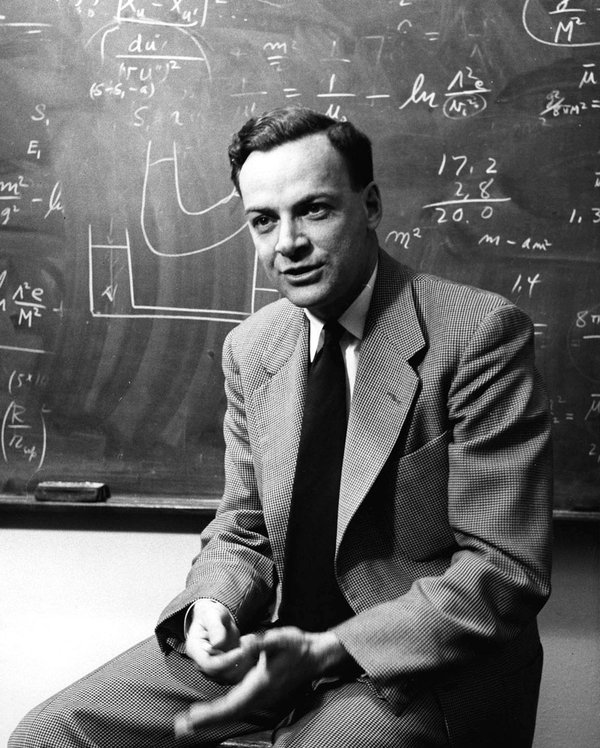
\includegraphics[width=2.5cm]{pics/feynman.jpg}
	}
}

~\\
~\\
~\\
~\\
\pause

		~~~~~~~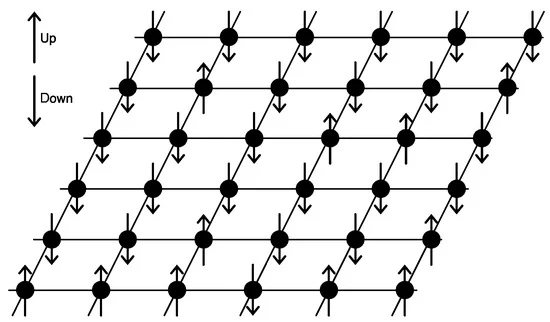
\includegraphics[width=4cm]{ising}
		
		Computing spins requires exponentially many calculations

\end{refframe}




\begin{refframe}{Quantum Computing}

	\begin{block}{\bf Feynman's conception: the quantum computer}
		\begin{itemize}
%%		\item Some evidence that quantum can solve classically intractable problems
%  		\item Nature is inherently quantum
%		\begin{itemize}
%  		\item Nowadays, physicists and chemists need to solve hard simulation problems
%  		\item Many problems physicists deal with are \QMA-complete (``Quantum \NP'')
%		\end{itemize}
%\pause
  		\item Turn the problem around: Let's make nature's complexity work for us
\pause
%  		\item Recent progress:
%		\begin{itemize}
  		\item Progress: Google's~\cite{arute2019quantum} and IBM's~\cite{kim2023evidence} quantum supremacy experiments
%  		\item IBM's quantum supremacy experiment
%		\end{itemize}
%		\item Classical hardware is reaching its limitations
%		\begin{itemize}
%  		\item Quantum effects, like tunneling, put a spoke in the wheel
%  		\item Philosophically interesting
%		\end{itemize}
		\end{itemize}
	\end{block}
	

	\centering

%\onslide<3->{	
%	\alert{The ultimate goal now is \textbf{quantum supremacy}:\\
%		a first, useful computation with an error-corrected quantum computer}
%}

\end{refframe}




%\begin{frame}{Physicists Use Tensor Networks}
%\end{frame}



\begin{refframe}{Quantum Computing Skepticism}

\vfill

\begin{alertblock}<+->{Obstacles}
		\begin{itemize}
		\item What if the (error-corrected) quantum computer never materializes?
\pause
		\item What if it turns out that \BQP{} = \P?
%		\item the device is too hard to build
		\end{itemize}
\end{alertblock}



\centering
\cols{
\col{.3\textwidth}{\centering
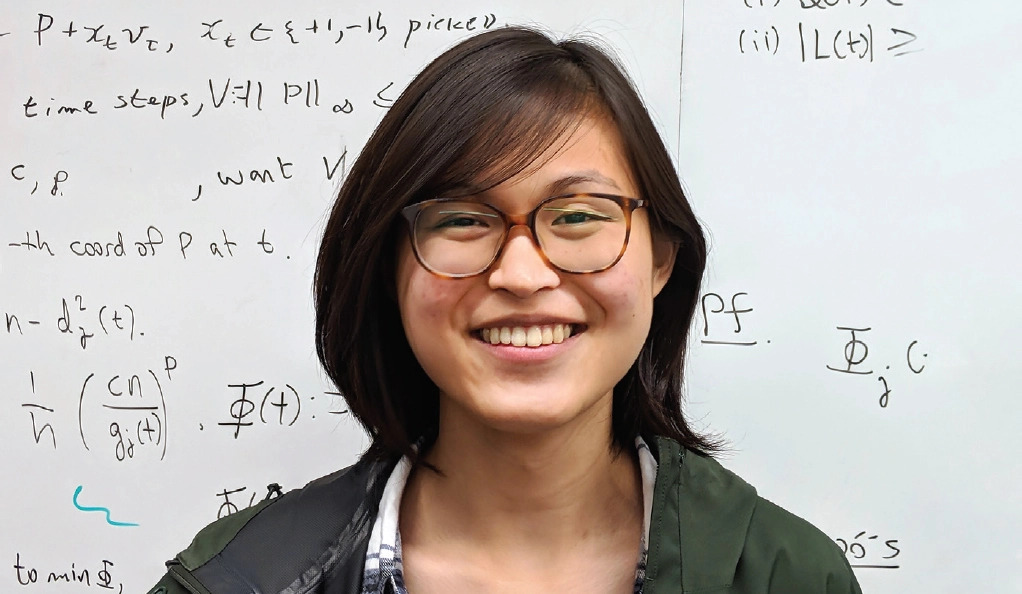
\includegraphics[width=3cm]{tang.jpeg}
}
\col{.7\textwidth}{
Ewin Tang~\cite{tang2019quantum} gave efficient classical algorithms for the recommender problem (at age 18)
}}

\onslide<+->{}

%\onslide<2->{
%\alert{Regardless of whether a quantum computer ever gets build, we are improving our understanding of quantum-hard problems.}
%}

%\vspace{-.5em}
\onslide<+->{
	\begin{block}{\bf Quantum computing Optimism}
		\begin{itemize}
%			\item The potential for exponential speedups
			\item<.-> There are (arguably) good arguments against this skepticism, but ...
%			We run into physical limitations (Moore's law), better use quantum effects
			\item<+-> \alert{Nature keeps posing ``quantum-hard'' questions}
		\begin{itemize}
		\item<.-> Cracking problems in quantum computing solves quantum-hard problems
		\item<.-> Applications in the simulation of physical systems, quantum chemistry, etc
%		\item the device is too hard to build
		\end{itemize}
		\item<+-> \alert{Our results with quantum circuits can be translated back to physics applications.}
		\end{itemize}	
	\end{block}
}


\onslide<.->{
\cols{
\col{.5\textwidth}{\centering
\hfill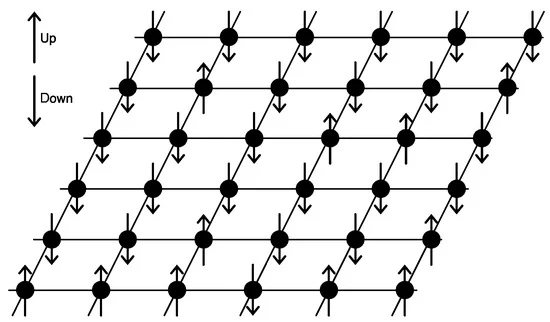
\includegraphics[width=2cm]{ising}~~~~~~~~~
}
\col{.5\textwidth}{\centering
~~
$
\scalebox{.8}{
\Qcircuit @C=1.em @R=.7em {
\lstick{\ket{0}} & & \gate{H}  & \ctrl{1} 						& \gate{H} 	& \qw      & \qw  \\
\lstick{ \longleftarrow ~~~~~~~~~~~\ket{0}} & &  \gate{H} & \gate{X} 						& \gate{H}  	& \ctrl{1} & \qw  &  \\
\lstick{\ket{0}} &  & \qw      & \push{\rule{1.5em}{.4pt}}\qw 	& \qw 	& \gate{X} & \qw  
}}
$
}}
}

\end{refframe}





\begin{frame}{On the Road to Quantum Supremacy}



	\begin{block}{\bf How can we contribute?}
		\begin{itemize}
		\item Build an (error-corrected) quantum computer
		\item<+-> Come up with a new quantum algorithm that shows that $\BQP \neq P$
		\item<+-> \alert{Invent the tools to use current and future quantum computers}
%\pause
%		\begin{itemize}
%		\item \alert{Comparing data structures for representing quantum information}
%		\item \alert{Quantum circuit compilation}
%		\item \alert{Simulation and analysis of physical systems}
%		\item \dots
%		\end{itemize}
		\end{itemize}
	\end{block}

\centering
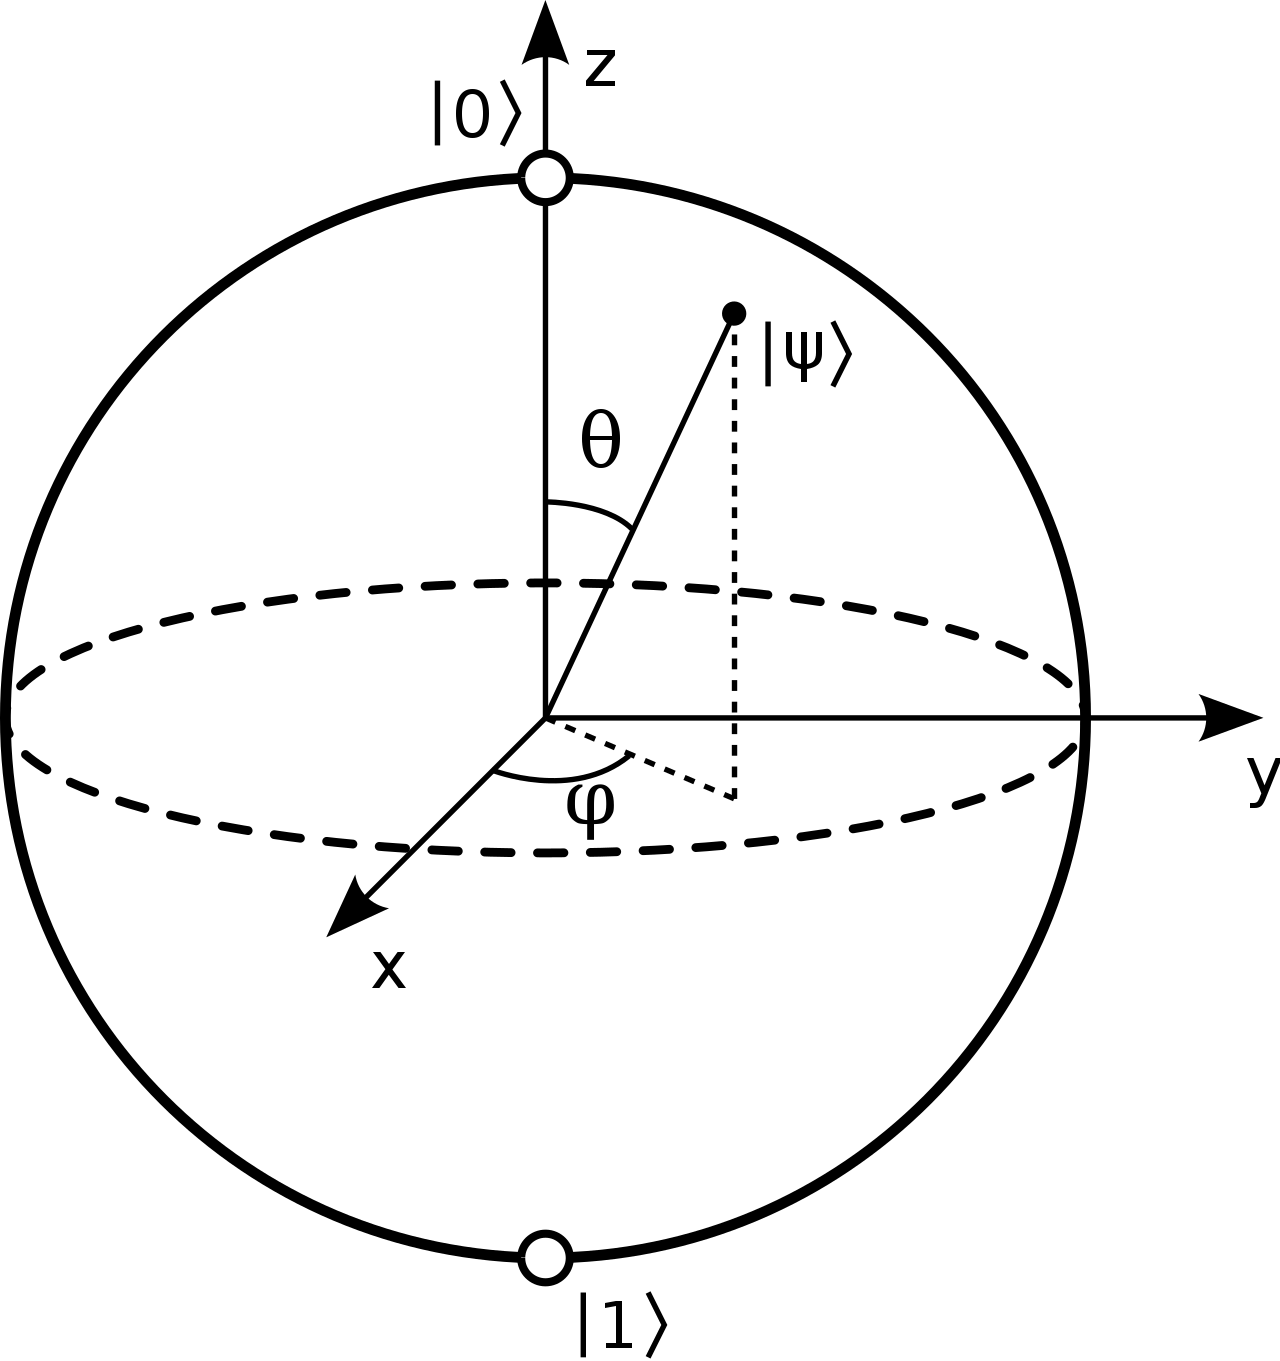
\includegraphics[width=3cm]{graphics/Bloch_sphere.svg.png}


\end{frame}







\begin{frame}{Quantum Circuit Compilation}


	\begin{block}{\bf Compilation is essential}
		\begin{itemize}
		\item Efficiently utilize early frugale quantum computers
%		\item ....
		\item Error correction requires hybrid solutions with fast classical components
		\end{itemize}
	\end{block}

\pause
\vspace{-.5em}

	\begin{block}{\bf Compilation entails...}
		\begin{itemize}%~\cite{burgholzer2020advanced,viamontes2003improving,vinkhuijzen2021limdd}
		\item<+-> Quantum circuit optimization
%		\begin{itemize}
%				\item match circuit to hardware topology,
%				\item gate type minimization,
%				\item space minimization,
%				\item depth minimization,
%		\end{itemize}
		\item<+-> Quantum circuit synthesis
%		\begin{itemize}
%				\item Given a description, generate a quantum circuit
%				\item Often with constraints as in optimization
%		\end{itemize}
%		\item Quantum circuit verification~\cite{}
		\item<+-> {\color{OliveGreen} Quantum circuit simulation}			\hfill (a subtask in various analyses)
		\item<+-> {\color{red} Quantum circuit equivalence checking}  \hfill (for checking correctness)%~\cite{thanos2023fast,peham2022equivalence}
			%~\cite{brand2023quantum,}
		\end{itemize}
	\end{block}

\vspace{-.8em}

\cols{
\col{1cm}{}
\col{4cm}{
\[
\scalebox{.8}{
\Qcircuit @C=1.em @R=.7em {
\lstick{\ket{0}} & & \gate{H}  & \ctrl{1} 						& \gate{H} 	& \qw      & \qw  \\
\lstick{\ket{0}} & &  \gate{H} & \gate{X} 						& \gate{H}  	& \ctrl{1} & \qw  & ~~~~~~~~~~~~~~~~~~\stackrel?=~~~~~~~~~ \\
\lstick{\ket{0}} &  & \qw      & \push{\rule{1.5em}{.4pt}}\qw 	& \qw 	& \gate{X} & \qw  
}}
\]
}
\col{3cm}{
\[
\scalebox{.8}{
\Qcircuit @C=1.em @R=.7em {
\lstick{\ket{0}} & & \qw &  \gate{X}						&\qw	& \qw      & \qw  \\
\lstick{\ket{0}} & & \qw      & \ctrl{- 1} 						&\qw 	& \ctrl{1} & \qw  \\
\lstick{\ket{0}} &  & \qw      & \push{\rule{1.5em}{.4pt}}\qw 	& \qw 	& \gate{X} & \qw  
}}
\]
}
\col{1cm}{}
}

%\centering
%Quantum Circuit Compilation

\end{frame}




%\begin{frame}{\large\hbox{\hspace{-1em} The Unreasonable Effectiveness of {\normalsize (Classical)} Automated Reasoning in Quantum}}
%	
%	\begin{block}{\bf In this survey:}
%		Highly successful applications of classical automated reasoning methods for the synthesis, simulation, and equivalence checking of circuits:
%		\begin{itemize}
%			\item Decision diagrams
%			\item SAT / SMT / \#SAT (model counting)
%			\item Diagrammatic languages (ZX calculus)
%		\end{itemize}
%	\end{block}
%	
%
%\pause
%
%	\begin{block}{\bf How is this even possible?}
%		\begin{itemize}
%			\item Discretization of the Hilbert space according to exact interpretation of circuits
%			\item Reinterpret quantum states as density matrices in suitable basis (Pauli)
%			\item Symbolic treatment of amplitudes / weights
%		\end{itemize}	
%	\end{block}
%	
%\end{frame}
%






\begin{frame}{Automated Reasoning in Quantum Circuit Compilation}

\vfill

\cols{
\col{5cm}{
	\begin{block}{\bf Automated Reasoning Method}
%\only<5->{\begin{enumerate}
%			\item[\alert{1.}] Decision diagrams
%			\item[\alert{2.}]  SAT / SMT / \#SAT
%			\item[\alert{3.}]  Diagrammatic languages
%		\end{enumerate}}
%\only<1-4>{	
	\begin{itemize}
			\item Decision diagrams
			\item SAT / SMT / \#SAT
%			\item Diagrammatic languages
		\end{itemize}
%		}
	\end{block}
}
\col{.5cm}{~\\\Huge $\times$}
\col{5cm}{
	\begin{block}{\bf Quantum Circuit Compilation}
		\begin{itemize}
		\item {optimization / synthesis}
		\item \color{OliveGreen}simulation
		\item \color{red}equivalence checking 
		\end{itemize}
	\end{block}
}}

\vfill

\pause

	\begin{block}{\bf Methodology}
		\begin{itemize}
		\item Top results from Google Scholar using appropriate keywords
		\item Literature review (follow the trail of citations)
		\item Check results with colleagues in FM and QC
		\end{itemize}
	\end{block}

\pause

\vfill


	\begin{alertblock}{\bf Methodology}
		\begin{itemize}
		\item Bias remains.. so I will discuss our own contributions separately.
		\pause
		\item Focus on advancing quantum, not on applying formal methods to quantum
		\end{itemize}
	\end{alertblock}



\end{frame}


\begin{frame}[noframenumbering]{Overview}


		\begin{enumerate}
			\item[0.] Quantum Computing \\~\\
			\item SAT-based methods
			\item DD-based methods
%			\item Diagrammatic languages
\\
~\\
			\item Translating results back Quantum Physics
		\end{enumerate}
\end{frame}


%\begin{frame}{Quantum Circuit Simulation}
%
%\vfill
%
%~~~~~~~~~~~~~~
%\Qcircuit @C=2.3em @R=0.7em {
%& \ket{0} & & \gate{H} & \ctrl{1} & \qw      & \qw  \\
%& \ket{0} & & \qw      & \gate{X} & \ctrl{1} & \qw \\
%& \ket{0} & & \qw      & \push{\rule{1.5em}{.4pt}}\qw & \gate{X} & \meter\\
%&	  & & \dstick{U_1} & \dstick{U_2} & \dstick{U_3}  	 & \dstick{U_4}
%\gategroup{1}{4}{3}{4}{.7em}{--}
%\gategroup{1}{5}{3}{5}{.7em}{--}
%\gategroup{1}{6}{3}{6}{.7em}{--}
%\gategroup{1}{7}{3}{7}{.7em}{--}
%}
%
%\vfill
%
%\vspace{1em}
%
%\pause
%\begin{exampleblock}{State-based simulation}
%\centering
%\scalebox{1.5}{
%$ \ket{\phi_1} ~~=~~ U_1 \cdot \ket{\phi_0} $
%}
%
%\scalebox{1.5}{
%$ \ket{\phi_2} ~~=~~ U_2 \cdot \ket{\phi_1} $
%}
%
%\scalebox{1.5}{
%$ \ket{\phi_3} ~~=~~ U_3 \cdot \ket{\phi_2} $
%}
%
%\scalebox{1.5}{
%$ \ket{\phi_4} ~~=~~ \hspace{-.07cm}\underbrace{U_4}_{\mathclap{\text{simple matrices}}}  \hspace{-.1cm} \cdot \ket{\phi_3} $
%}
%\end{exampleblock}
%
%\pause
%
%\begin{block}{Strong vs weak simulation}
%	\begin{itemize}
%		\item \textbf{Strong}: compute probability $\braket{b | \phi_3}$ of the measure outcome  for any $b\in \set{0,1}^n$
%		\item \textbf{Weak}: sample the probability distribution $b\in \set{0,1}^n \to \braket{b | \phi_3}$
%
%			\alert{(This is what a quantum computer does.)}
%	\end{itemize}
%\end{block}
%
%
%\vfill
%	
%\end{frame}


%\begin{refframe}{Verification: Circuit Equivalence Checking}
%
%\vfill
%
%\centering
%
%
%\begin{columns}
%\begin{column}{.05\textwidth}
%\end{column}
%\begin{column}{.4\textwidth}
%\scalebox{1}{
%\Qcircuit @C=1.em @R=.7em {
%& & \gate{H} & \ctrl{1} 						&\qw	& \qw      & \qw  \\
%& & \qw      & \gate{X} 						&\qw 	& \ctrl{1} & \qw  \\
%&  & \qw      & \push{\rule{1.5em}{.4pt}}\qw 	& \qw 	& \gate{X} & \qw  
%}}
%\end{column}
%\begin{column}{.08\textwidth}
%\hspace{-.em}
%\scalebox{2}{$\stackrel?\approx$}
%\end{column}
%\begin{column}{.4\textwidth}
%\scalebox{1}{
%\Qcircuit @C=1em @R=.7em {
%& & \qw		  &  \gate{X}  						& \gate{H} 	& \qw      & \qw  \\
%& & \gate{H}  &  \ctrl{-1}\qwx[0] 				& \gate{H} 	& \ctrl{1} & \qw \\
%&  & \qw      & \push{\rule{1.5em}{.4pt}}\qw  	&\qw  		&   \gate{X}&\qw  
%}}
%\end{column}
%\begin{column}{.05\textwidth}
%\end{column}
%\end{columns}
%
%\vspace{.5cm}
%
%
%\pause
%
%
%We can reduce this problem to \alert{strong} simulation \cite{thanos2023fast}.
%
%(A reduction to weak simulation would imply ``Quantum \P'' = ``Quantum \NP'')
%
%\end{refframe}





\begin{frame}
\vfill


\Large

\begin{quote}
``Quantum computing becomes easy once you take the physics out of it''
\end{quote}
\hfill
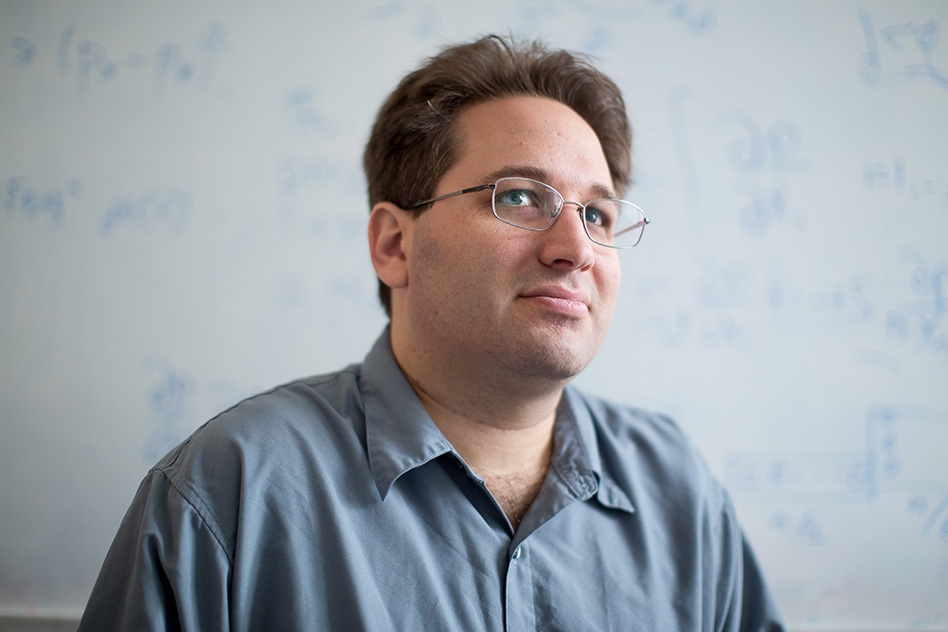
\includegraphics[width=5cm]{scott-aaronson.jpeg}

\hfill Scott Aaronson

\pause

\vfill

\begin{quote}
``Quantum computing becomes \only<1>{easy}\only<2>{\underline{even easier}} once you take the \only<2>{\underline{most linear algebra}} out of it''
\end{quote}
\hfill Alfons Laarman
%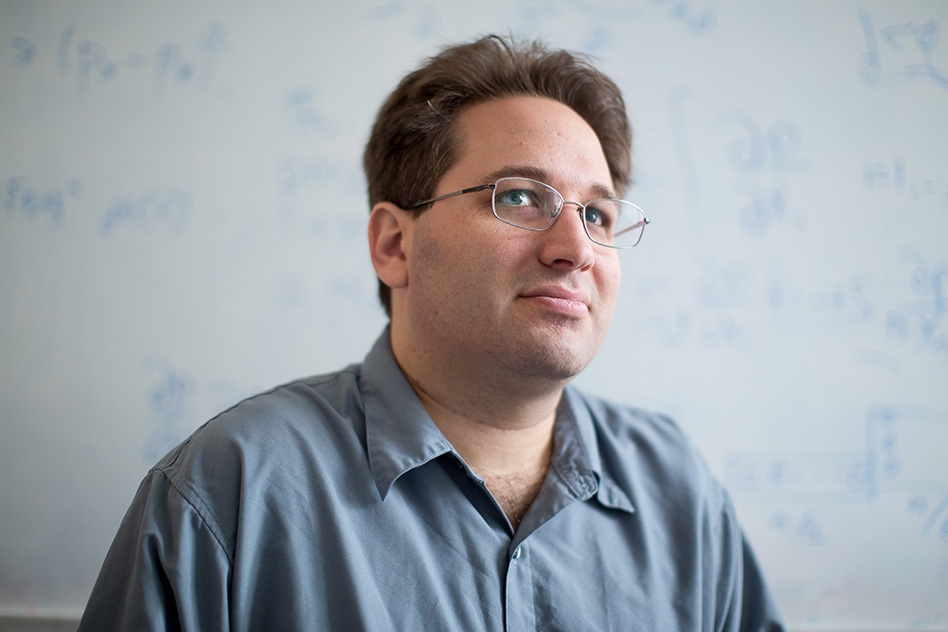
\includegraphics[width=5cm]{scott-aaronson.jpeg}


%\hfill \url{https://scottaaronson.blog}
\end{frame}




\begin{frame}{Quantum State}

%\centering

\[ \scalebox{2}{$ \vec v  = $} %\ket\phi \pause =
	\def\arraystretch{1.3}
    \onslide<2->{
    \begin{matrix*}[c]
    \text{index }\overbrace{000\dots000}^{\mathclap{\text{\alert{computational basis state}}}}:\\\text{index }{000\dots001}:\\\text{index }{000\dots010}:\\\text{index }{000\dots011}:\\\vdots\vspace{1em}\\\\\text{index }\underbrace{111\dots111}_{\vspace{3em}}:\\
    \end{matrix*}
    }
    \left.
    \begin{bmatrix*}[c]
     i \\0 \\ 0\\ 0 \\ \vdots \\ 0 \\ 0\\ 0  \\
    \end{bmatrix*}
    \right\}\text{ $2^n$ complex \alert{probability amplitudes}}
\]


\pause[4]
%\centering
%\alert{A quantum state is a pseudo-Boolean function:  $\set{0,1}^n\to \complex$}

\centering
\begin{tikzpicture}\footnotesize
  \tikzset{venn circle/.style={circle,minimum width=2cm,fill=####1,opacity=0.4}}
  \node [venn circle=white,minimum width=2.5cm,draw] (A) at (0,0.3) {};
  \node  at (0,1.25) 			{Quantum states};

%  \node [venn circle = Red!40!white, ellipse,minimum height=2.2cm, minimum width=3.6cm] (L) at (0,0.6) {};
%  \node  at (0,1.5) 		{\limdd};
  
%  \node [venn circle = blue!70!white,text width=1.3cm,align=center,rotate=79,ellipse,minimum height=1.8cm, minimum width=2.5cm] (B) at (-.6,-.2) {};
%  \node[text width=1.3cm,align=center]  at (-.9,-1.) {MPS};


%  \node [venn circle = green!70!white,text width=1.3cm,align=center,rotate=119,ellipse,minimum height=1.8cm, minimum width=2.5cm] (B) at (.6,-.2) {};
%  \node[text width=1.3cm,align=center]  at (.9,-1.) {RBM};



%  \node [venn circle = Blue!100!white,text width=1cm,align=center, minimum width=1.cm] (B) at (-.5,.3) 	{\textcolor{white}{QMDD}};						

  \node [venn circle = OliveGreen,text width=1cm,align=center, minimum width=.8cm,opacity=.5,text opacity=1] (C) at (.5,.2) {\textcolor{white}{Stabilizer states}};
\end{tikzpicture}	

\alert{Stabilizer circuits are non-universal \& classically simulatable, but crucial in error correction, etc.}

\end{frame}



\begin{frame}{Quantum Gate / Circuit}
	
\centering 

\scalebox{.7}{
\begin{circuitikz}
\draw
(0,2) node[and port] (myand) {\hspace{-1ex}$\land$}
(2,1) node[or port] (myor) {\hspace{-1ex}$\lor$}
(myand.in 1) node[anchor=east] {$a$}
(myand.in 2) node[anchor=east] (bnode) {$b$}
(myand.out) -| node[above]{$x$} (myor.in 1)
node[below=.638cm of bnode] (cnode) {$c$}
(cnode) -|  (myor.in 2)
(myor.out) node[anchor=west] {$y$}
;
\end{circuitikz}
}

\pause

\vspace{-2ex}
\[
\scalebox{1}{
\Qcircuit @C=1em @R=.2em @!R {
\lstick{\ket{a}_a} & & \qw &  \ctrl{2} 	&\qw	& \qw      & \qw  \\
\lstick{\ket{b}_b} & & \qw &  \ctrl{1}	&\qw 	& \qw      & \qw  \\
\lstick{\ket{0}_x} &  & \qw & \targ  &\qw 	    & \ctrlo{1} & \qw \\  
\lstick{\ket{c}_c} & & \qw &     \qw 	&\qw	& \ctrlo{1} & \qw  \\
\lstick{\ket{1}_y} &  & \qw &     \qw   &\qw 	& \targ & \qw 
%\onslide<4->{ \gategroup{1}{3}{5}{5}{.7em}{--} }
}}
\]


\pause

%\[
%\scalebox{1}{
%\Qcircuit @C=1em @R=.2em @!R {
%\lstick{\ket{a}_a} & & \qw &  \ctrl{2} 	&\qw	& \qw      & \qw  \\
%\lstick{\ket{b}_b} & & \qw &  \ctrl{1}	&\qw 	& \qw      & \qw  \\
%&&\dots&&&\\
%\lstick{\ket{c}_c} & & \qw &     \qw 	&\qw	& \ctrlo{1} & \qw  \\
%\lstick{\ket{1}_y} &  & \qw &     \qw   &\qw 	& \targ & \qw  
%}}
%\]


$
\underbrace{
\begin{bmatrix}
1 & 0  & \dots & -i\\
%\pm P_{2,1}}:& P_{2,2}~~~  \otimes& \dots & \otimes~~~ P_{2,n},\\
\vdots  & \vdots  & \ddots& \vdots\\
i & 0  & \dots &  1\\
\end{bmatrix}
}_{2^n}
\left.
\hspace{-1ex}
\vphantom{
\begin{bmatrix}
1 & 0  & \dots & -i\\
%\pm P_{2,1}}:& P_{2,2}~~~  \otimes& \dots & \otimes~~~ P_{2,n},\\
\vdots  & \vdots  & \ddots& \vdots\\
i & 0  & \dots &  1\\
\end{bmatrix}}
\right\}\text{\scriptsize $2^n$}
$

~\\

\pause

Simulation of quantum circuits: $G_k \cdots G_1 \cdot \vec v$

\end{frame}




%\begin{frame}{Classical vs Quantum Information}
%%	\framesubtitle{The proof uses \textit{reductio ad absurdum}.}
%
%\hspace{-2em}
%\renewcommand\arraystretch{2}
%\begin{tabular}{r|p{3.7cm}|p{5cm}}
%				& \textbf{Classical} & \bf Quantum \\\hline
%\textit{Unit:} 	& Bit		& Qubit \\
%\pause
%\textit{State:}  & Bitvector: $\vec s \in \set{0,1}^n$
%	 & Pseudo-Boolean function:  $\set{0,1}^n\to \complex$ \\
%\pause
%\textit{Example:}  & 
%$\underbrace{(0,0, 1, \dots, 1, 1, 0)}_{\text{length $n$}}$
%&
%%~~~~$\overbrace{}^{\dots 000}$\vspace{-1ex}
%$
%\tfrac1{\sqrt 3}
%\underbrace{
%[
%    i, 0, 0, 0,  \dots \dots \dots \dots \dots \dots, 0, 1, 0, i
%]^T
%}_{\text{complex vector of \alert{length $2^n$}}}
%$  
% \\
%%\onslide<4->{
%\textit{Model:}  & (Uniform) Boolean circuits 
%
%\scalebox{.7}{
%\begin{circuitikz}
%\draw
%(0,2) node[and port] (myand) {\hspace{-1ex}$\land$}
%(2,1) node[or port] (myor) {\hspace{-1ex}$\lor$}
%(myand.in 1) node[anchor=east] {$a$}
%(myand.in 2) node[anchor=east] (bnode) {$b$}
%(myand.out) -| node[above]{$x$} (myor.in 1)
%node[below=.638cm of bnode] (cnode) {$c$}
%(cnode) -|  (myor.in 2)
%(myor.out) node[anchor=west] {$y$}
%;
%\end{circuitikz}
%}
%& (Uniform) quantum circuits 
%
%\vspace{-2ex}
%\[
%\scalebox{1}{
%\Qcircuit @C=1em @R=.2em @!R {
%\lstick{\ket{a}_a} & & \qw &  \ctrl{2} 	&\qw	& \qw      & \qw  \\
%\lstick{\ket{b}_b} & & \qw &  \ctrl{1}	&\qw 	& \qw      & \qw  \\
%\lstick{\ket{0}_x} &  & \qw & \targ  &\qw 	    & \ctrlo{1} & \qw \\  
%\lstick{\ket{c}_c} & & \qw &     \qw 	&\qw	& \ctrlo{1} & \qw  \\
%\lstick{\ket{1}_y} &  & \qw &     \qw   &\qw 	& \targ & \qw  
%}}
%\]
%\\
%\pause
%&&
%~~~~~~~~~~~$
%\underbrace{
%\begin{bmatrix}
%1 & 0  & \dots & -i\\
%%\pm P_{2,1}}:& P_{2,2}~~~  \otimes& \dots & \otimes~~~ P_{2,n},\\
%\vdots  & \vdots  & \ddots& \vdots\\
%i & 0  & \dots &  1\\
%\end{bmatrix}
%}_{2^n}
%\left.
%\hspace{-1ex}
%\vphantom{
%\begin{bmatrix}
%1 & 0  & \dots & -i\\
%%\pm P_{2,1}}:& P_{2,2}~~~  \otimes& \dots & \otimes~~~ P_{2,n},\\
%\vdots  & \vdots  & \ddots& \vdots\\
%i & 0  & \dots &  1\\
%\end{bmatrix}}
%\right\}\text{\scriptsize $2^n$}
%$
%
%
%
%\end{tabular}
%\end{frame}




%\begin{frame}{Quantum Information: Stabilizer Formalism}
%%	\framesubtitle{The proof uses \textit{reductio ad absurdum}.}
%
%\hspace{-2em}
%\renewcommand\arraystretch{1.7}
%\begin{tabular}{r|p{3.7cm}|p{5cm}|}
%				& \textbf{Stabilizer} & \bf Quantum \\\hline
%\textit{Unit:} 	& Qubit		& Qubit \\
%\pause
%\textit{State:}  & $n\times 2n$ bit matrix
%	 & Pseudo-Boolean function:  $\set{0,1}^n\to \complex$ \\
%\pause
%\textit{Example:}  & 
%$
%\renewcommand\arraystretch{1.}
%\left[
%\begin{matrix}
%00  & 01  & \dots & 11\\
%%\pm P_{2,1}}:& P_{2,2}~~~  \otimes& \dots & \otimes~~~ P_{2,n},\\
%\vdots  & \vdots  & \ddots& \vdots\\
%10 & 00  & \dots &  11\\
%\end{matrix} 
%\right]$
%&
%%~~~~$\overbrace{}^{\dots 000}$\vspace{-1ex}
%$
%\tfrac1{\sqrt 3}
%\underbrace{
%[
%    i, 0, 0, 0,  \dots \dots \dots \dots \dots \dots, 0, 1, 0, i
%]
%}_{\text{complex vector of \alert{length $2^n$}}}
%$  
% \\
%\pause
%\textit{Model:}  & (Uniform) \alert{Clifford} circuits 
%\vspace{-2ex}
%\[
%\scalebox{1}{
%\Qcircuit @C=1em @R=.em @!R {
%\lstick{\ket{0}} & & \qw &  \ctrl{1} 	&\qw	& \qw      & \qw  \\
%\lstick{\ket{0}} &  & \qw & \targ  &\qw 	   & \qw  & \qw \\  
%%\lstick{\ket{0}} & & \qw &     \qw 	&\qw	&\targ  & \qw  \\
%\lstick{\ket{0}} &  & \gate{H}  &     \qw   &\qw 	& \qw& \qw  
%}}
%\]
%& (Uniform) quantum circuits 
%\vspace{-2ex}
%\[
%\scalebox{1}{
%\Qcircuit @C=1em @R=.em @!R {
%\lstick{\ket{0}} & & \qw       &  \ctrl{2} 	&\qw	& \qw      & \qw  \\
%\lstick{\ket{0}} & & \qw       &  \ctrl{1}	&\qw 	& \qw      & \qw  \\
%\lstick{\ket{0}} &  & \gate{H} & \targ  &\qw 	    & \qw & \qw \\  
%%\lstick{\ket{0}} & & \gate{H} &     \qw 	&\qw	& \targ & \qw  \\
%}}
%\]
%\\
%\textit{Gate set:}& Clifford = \set{H, S, CX} & Clifford+$T$, Clifford+Toffoli, Clifford+.. \\
%\end{tabular}
%
%
%\cols{
%\col{5cm}{
%\alert{Clifford circuits are classically simulatable, but non-universal!}
%}
%\col{5cm}{
%\begin{tikzpicture}\footnotesize
%  \tikzset{venn circle/.style={circle,minimum width=2cm,fill=####1,opacity=0.4}}
%  \node [venn circle=white,minimum width=2.5cm,draw] (A) at (0,0.3) {};
%  \node  at (0,1.25) 			{Quantum states};
%
%%  \node [venn circle = Red!40!white, ellipse,minimum height=2.2cm, minimum width=3.6cm] (L) at (0,0.6) {};
%%  \node  at (0,1.5) 		{\limdd};
%  
%%  \node [venn circle = blue!70!white,text width=1.3cm,align=center,rotate=79,ellipse,minimum height=1.8cm, minimum width=2.5cm] (B) at (-.6,-.2) {};
%%  \node[text width=1.3cm,align=center]  at (-.9,-1.) {MPS};
%
%
%%  \node [venn circle = green!70!white,text width=1.3cm,align=center,rotate=119,ellipse,minimum height=1.8cm, minimum width=2.5cm] (B) at (.6,-.2) {};
%%  \node[text width=1.3cm,align=center]  at (.9,-1.) {RBM};
%
%
%
%%  \node [venn circle = Blue!100!white,text width=1cm,align=center, minimum width=1.cm] (B) at (-.5,.3) 	{\textcolor{white}{QMDD}};						
%
%  \node [venn circle = OliveGreen,text width=1cm,align=center, minimum width=.8cm,opacity=.5,text opacity=1] (C) at (.5,.2) {\textcolor{white}{Stabilizer states}};
%\end{tikzpicture}					
%}
%}
%
%\end{frame}




\begin{refframe}{Classical vs Quantum Computation}
%	\framesubtitle{The proof uses \textit{reductio ad absurdum}.}

\vfill

\tikzset{venn circle/.style={circle,minimum width=2cm,fill=####1,opacity=0.4}}
\begin{tikzpicture}[
e/.style = {ellipse, fill=####1, draw=none,
            minimum height=.7cm, minimum width=.9cm, inner sep=0pt},
e/.default=black
]
\footnotesize


%\draw[help lines] (0,0) grid (4,3);

\onslide<7->{
  \node [e = yellow!0!red!80!white,text width=2.8cm,align=center, minimum width=.8cm,  minimum height=3.6cm,text opacity=1,label={[anchor=north, inner sep=3pt,yshift=-.25cm]north:Precise\QMA = \PSPACE}] (PSPACE) at (.8,0.5) {};
	\node[right = of PSPACE.north east] (ECEQ) {\color{red} \textbf{Exact} quantum circuit non-equivalence};
	\draw[-Circle,shorten >= -.2cm] (ECEQ) -- (PSPACE.north east);
}


\onslide<6->{
  \node [e = yellow!30!red!80!white,text width=2.3cm,align=center, minimum width=.8cm,  minimum height=2.8cm,text opacity=1,label={[anchor=north, inner sep=3pt,yshift=-.2cm]north:Precise\BQP = \PP}] (PP) at (.8,0.3) {};
	\node[right = of PP.north east] (EQCSIM) {\color{OliveGreen} \textbf{Exact} quantum circuit simulation};
	\draw[-Circle,shorten >= -.2cm] (EQCSIM) -- (PP.north east);
}


\onslide<5->{
  \node [e = yellow!40!red!50!white,text width=2cm,align=center, minimum width=.8cm,  minimum height=2cm,text opacity=1,label={[anchor=north, inner sep=3pt]north:\QMA}] (QMA) at (.75,0.1) {};
	\node[right = of QMA.north east] (CEQ) {\color{red} Quantum circuit non-equivalence};
	\draw[-Circle,shorten >= -.2cm] (CEQ) -- (QMA.north east);
}


	\node [venn circle = yellow!80!red,text width=1cm,align=center, minimum width=.8cm,opacity=.5,text opacity=1,label={[anchor=west, inner sep=3pt]north west:\NP}] (NP) at (0,0) {};
	\node[left = of NP] (SAT) {\color{red}  Circuit non-equivalence};
	\draw[-Circle,shorten >= -.18cm] (SAT) -- (NP);
  
  
	\node<3-> [e = blue!80!white, opacity=0.5, minimum height=1cm] (BQP) at (1,0) {~~~~~~~~~~~~~~~\BQP};
  \node<4->[below right = of BQP,text width=3cm] (QCS) {\color{OliveGreen} Quantum circuit simulation};
  \draw<4->[-Circle,shorten >= -.18cm] (QCS) -- (BQP);
	
	
	\node<2-> [e = blue!60!white, opacity=.7] at (.5,0) {~~~~~~\BPP};


  \node [venn circle = blue!80,text width=.3cm,align=center, minimum width=.3cm,opacity=.5,text opacity=1] (P) at (.2,0) {{~~\P}};  
  \node[below left = of P] (CVP) {\color{OliveGreen} Circuit evaluation (simulation)};
  \draw[-Circle,shorten >= -.18cm] (CVP) -- (P);


%
%	\node<9->[below = of P.south,text width=4cm] (Clifford) {\centering \color{blue} Clifford circuit simulation \cite{aaronson2008improved} /\\ Clifford circuit non-equivalence \cite{ours}};
%	\draw<9->[-Circle,shorten >= -.2cm] (Clifford) -- (P.south);

\end{tikzpicture}					



\pause[8]

\centering
\vfill


	\begin{block}{Despite hardness, we often focus on exact methods!}
\begin{itemize}
	\item This enables symbolic computation
	\item We can solve approximate problems using exact methods~\cite{wei2022accurate,hong2021approximate}.
\end{itemize}
	\end{block}

\end{refframe}















